\newpage
\appendix
\section{Anhang}

\subsection*{Beispielrechnung aus Kapitel \ref{ssub:Klassifizierung} mit minsupport = 0.3} \label{anhang:zusatz1}

\begin{minipage}[t]{\textwidth}
%\begin{table}
	\begin{tabular}{c|c}
		$w_1$&0.6\\ \hline
		$w_2$&0.8\\ \hline
		$w_3$&0.4\\ \hline
		$w_4$&0.2\\ \hline
		$w_5$&0.6\\ 
	\end{tabular}
%\end{table}
	$\xrightarrow{\text{prüfe minsupport}}$
%\begin{table}
	\begin{tabular}{c|c}
		$w_1$&0.6\\ \hline
		$w_2$&0.8\\ \hline
		$w_3$&0.4\\ \hline
		$w_4$&0.2\\ 
	\end{tabular}
%\end{table}
	$\xrightarrow{\text{join Itemsets (prune ergibt keine Änderung)}}$
	\begin{tabular}{c|c}
		$w_1,w_2$&0.4\\ \hline
		$w_1,w_3$&0.2\\ \hline
		$w_1,w_5$&0.2\\ \hline
		$w_2,w_3$&0.2\\ \hline
		$w_2,w_5$&0.6\\ \hline
		$w_3,w_5$&0.2\\
	\end{tabular}
\end{minipage}
\newline
\newline
\begin{minipage}[t]{\textwidth}
%\begin{table}
%\end{table}
	$\xrightarrow{\text{prüfe minsupport}}$
%\begin{table}
	\begin{tabular}{c|c}
		$w_1,w_2$&0.4\\ \hline
		$w_2,w_5$&0.6\\ 
	\end{tabular}
%\end{table}
	$\xrightarrow{\text{join Itemsets}}$
	%\begin{tabular}{c|c}
		$\{w_1,w_2,w_5\}$
	%\end{tabular}
\end{minipage}\\
\newline
\newline
Da $w_1, w_5$ nicht häufig ist, ist auch $\{w_1,w_2,w_5\}$ nicht häufig. Somit sind $w_1,w_2$ und $w_2,w_5$ die gefundenen häufigen Itemsets..


\clearpage

\section{Pie Diagramme}
%\subsection*{Zusatzteil 2}
\label{anhang:zusatz2}
\begin{figure}[htb]
\begin{center}
	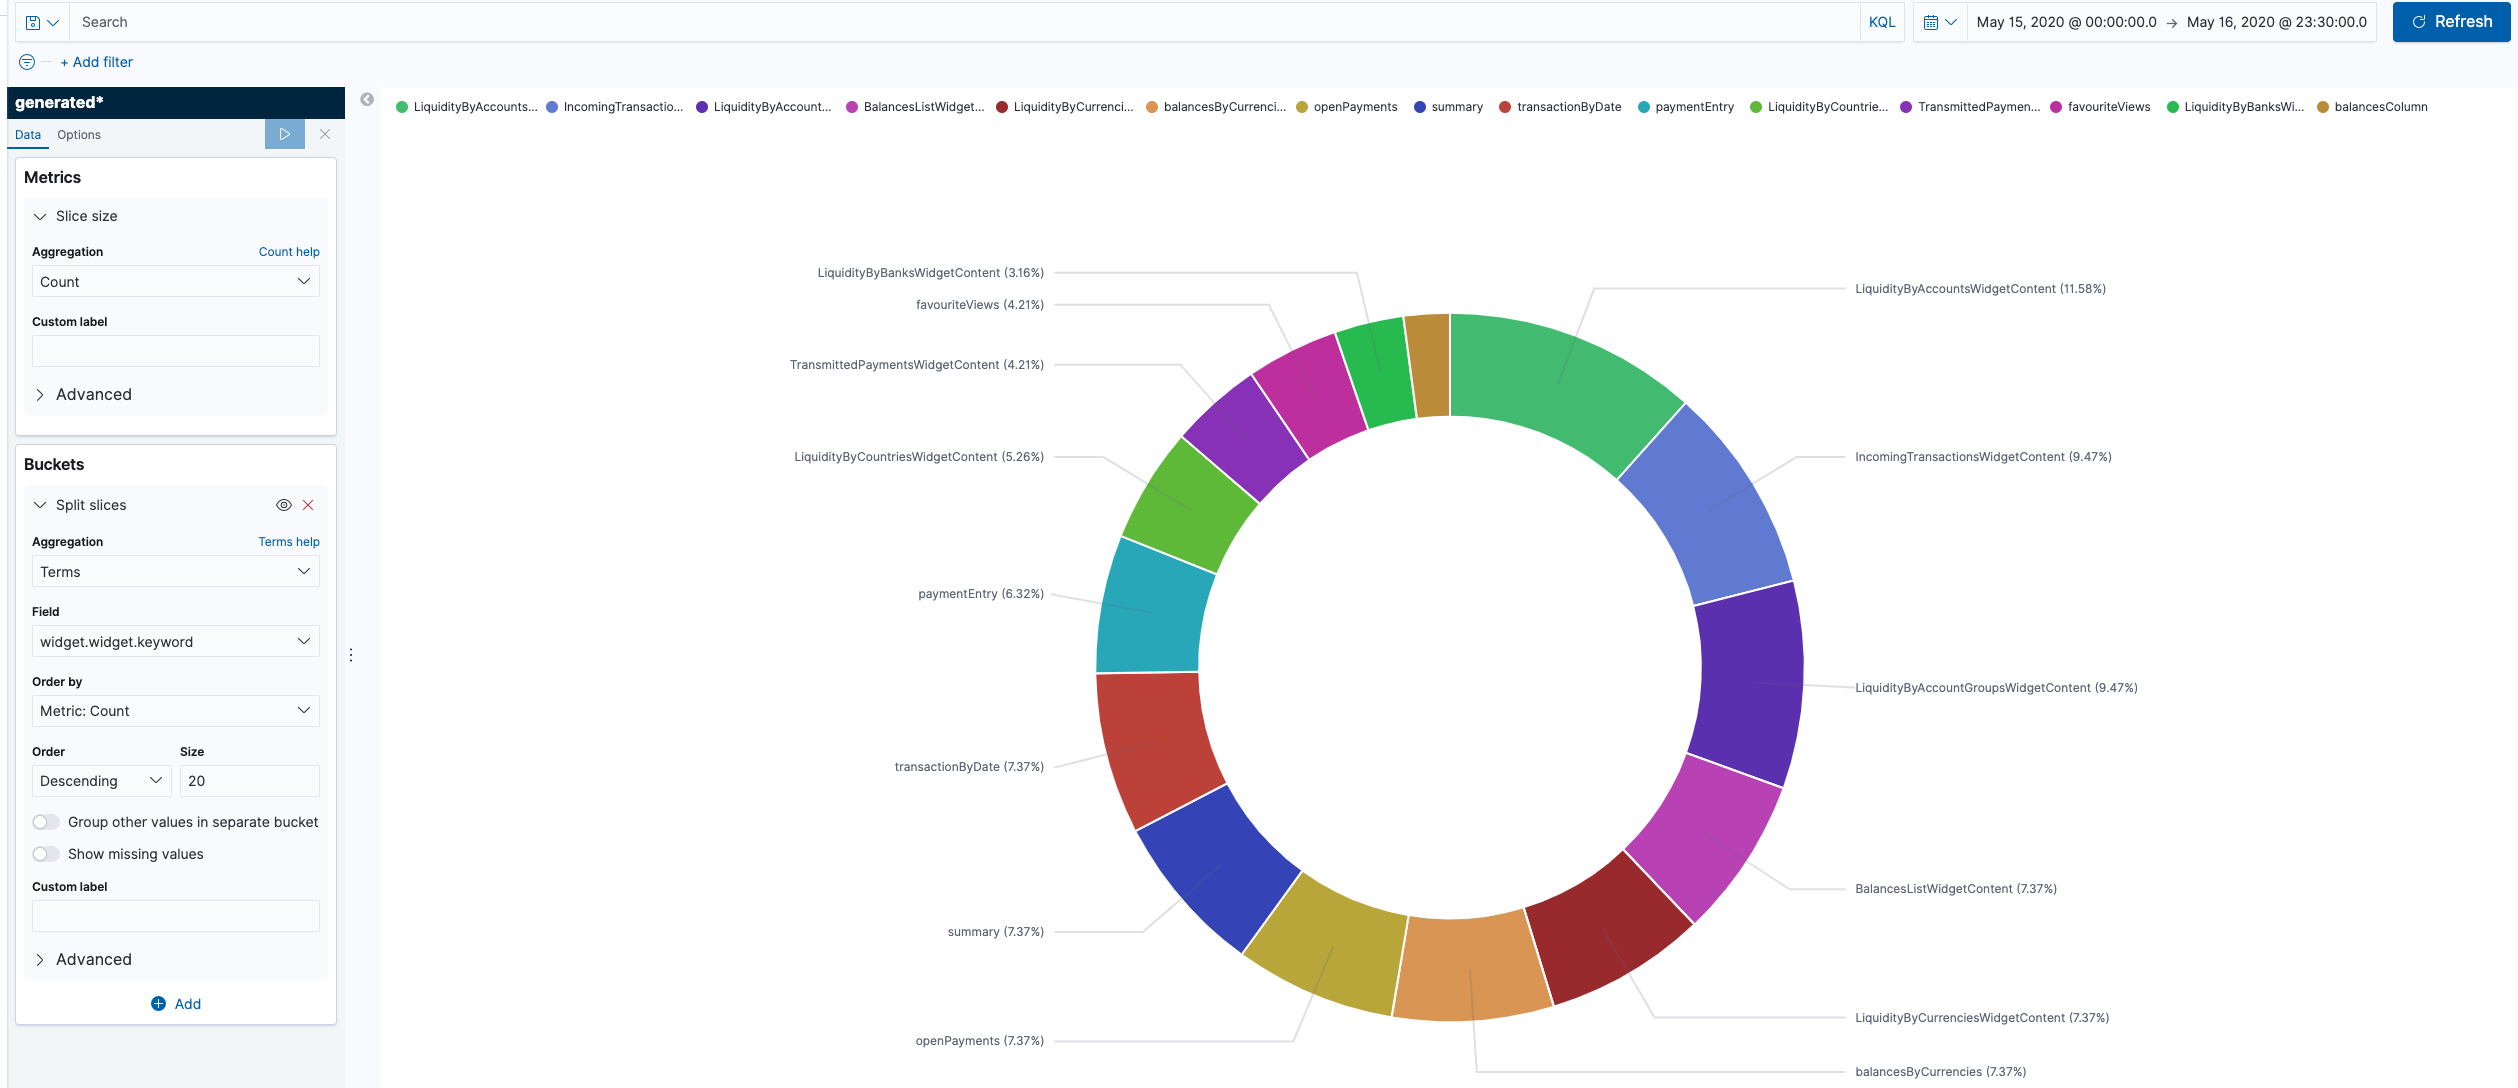
\includegraphics[width=430pt]{bilder/generated-pie.png}
\end{center}
\caption{Pie Visualisierung der generierten Daten}
\label{fig:generated-pie}
\end{figure}

\begin{figure}[htb]
\begin{center}
	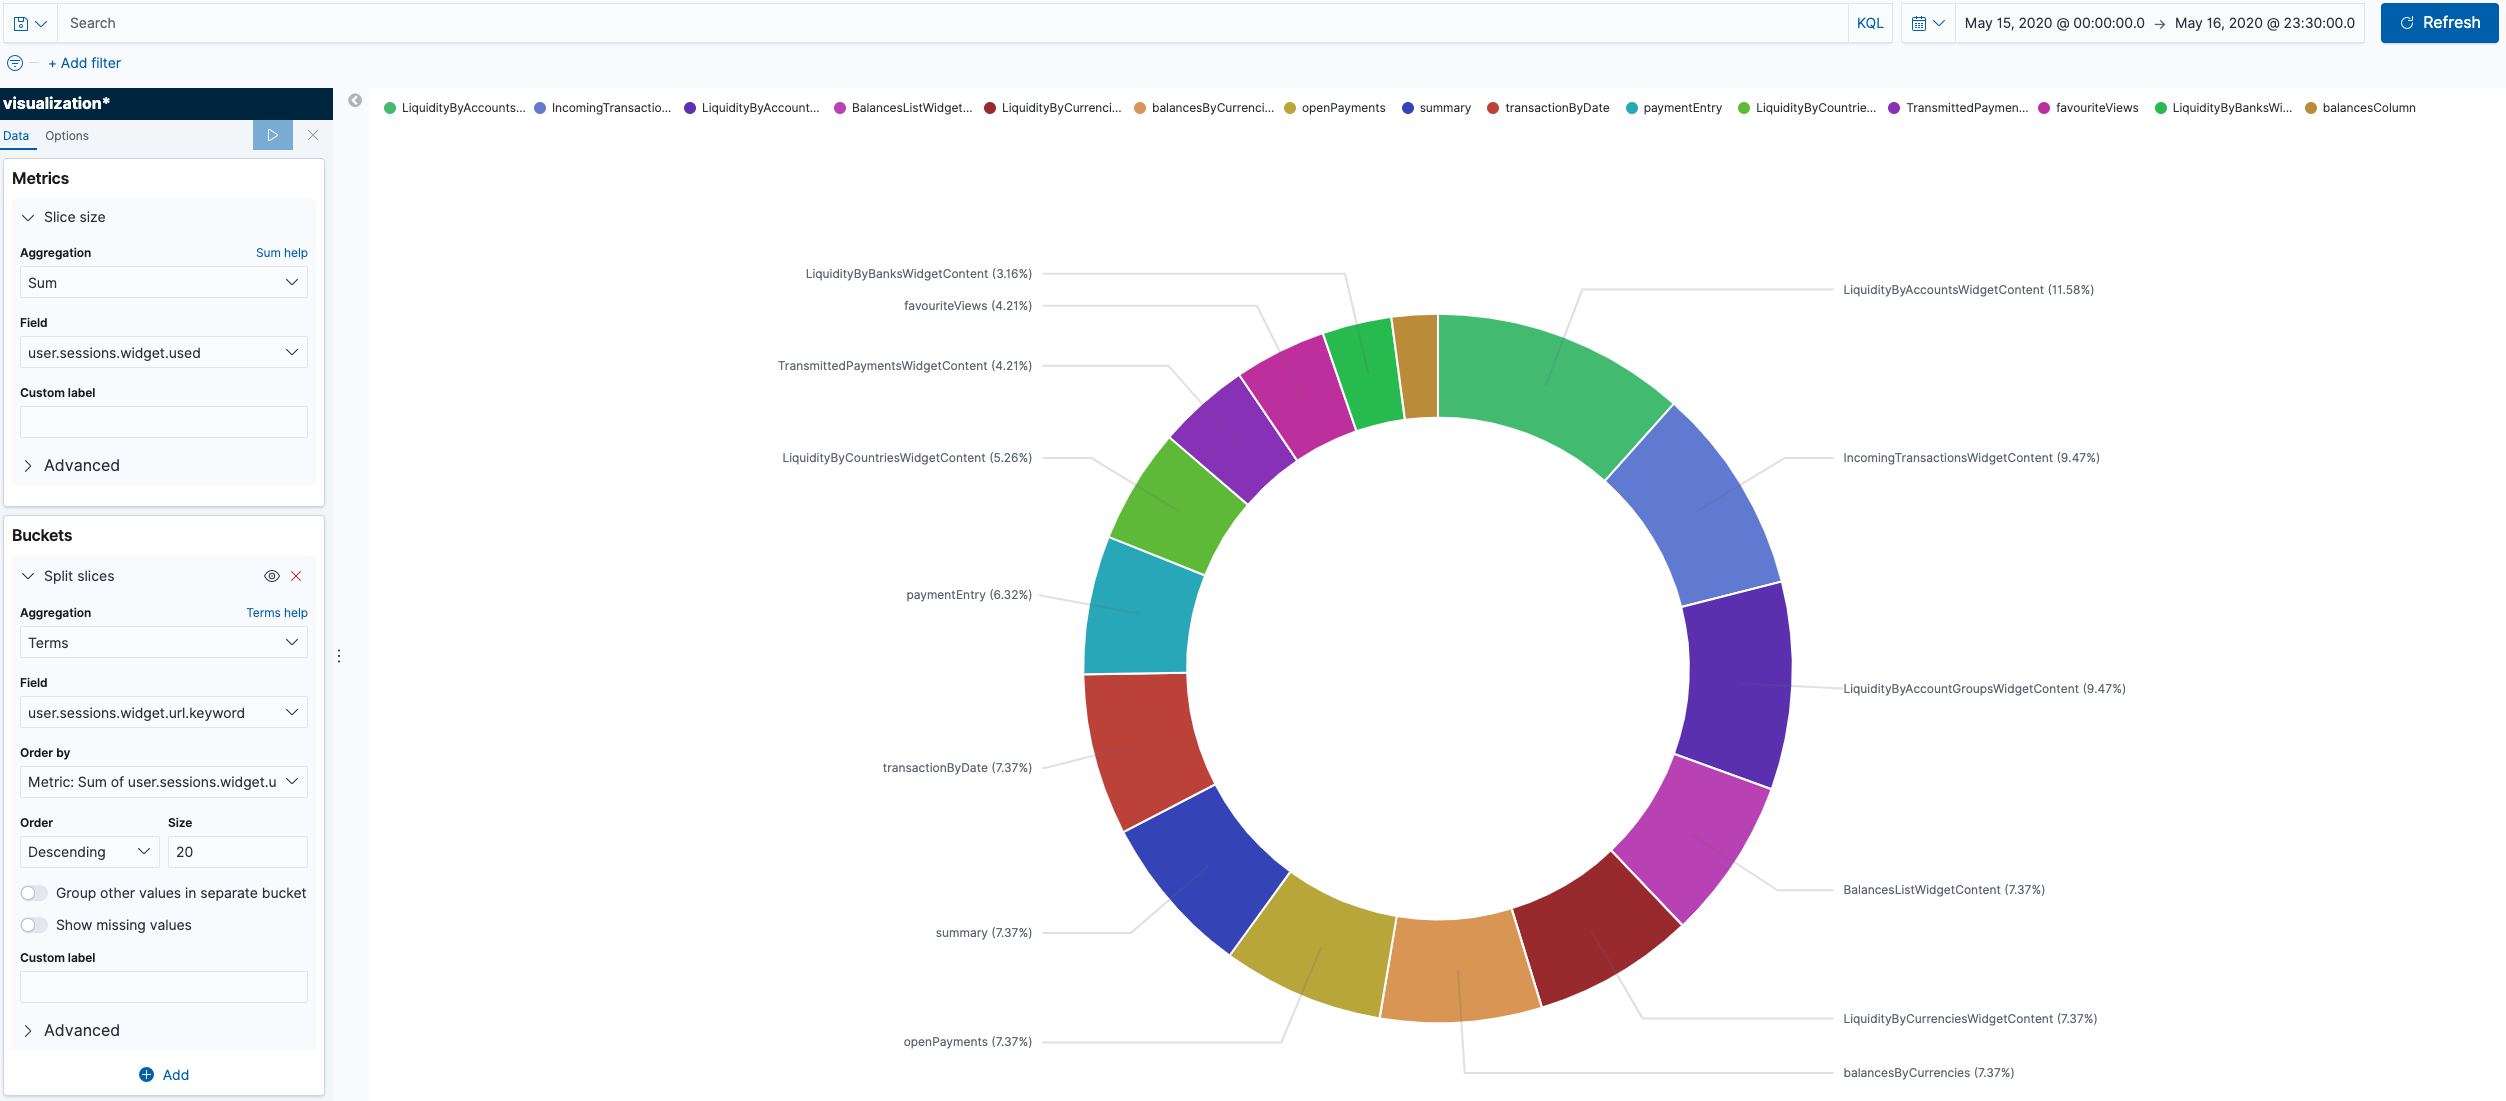
\includegraphics[width=430pt]{bilder/transformed-pie.png}
\end{center}
\caption{Pie Visualisierung der transformierten Daten}
\label{fig:transformed-pie}
\end{figure}



\clearpage
